\section{Câu hỏi 1: Xu hướng và mùa vụ}

Trung bình tháng thấp nhất là tháng \MonthlyMinMonth{} (\MonthlyMinValue{} m³/s), cao
nhất là tháng \MonthlyMaxMonth{} (\MonthlyMaxValue{} m³/s); biên độ trung bình tháng
chỉ khoảng 7,84 m³/s. Trong khi đó, trung bình năm thấp nhất là \YearlyMinYear{}
(\YearlyMinValue{} m³/s) và cao nhất là \YearlyMaxYear{} (\YearlyMaxValue{} m³/s),
biên độ tới 282,57 m³/s. Biến thiên giữa các năm lớn hơn nhiều so với biên độ mùa vụ
trung bình.

\begin{figure}[H]
\centering
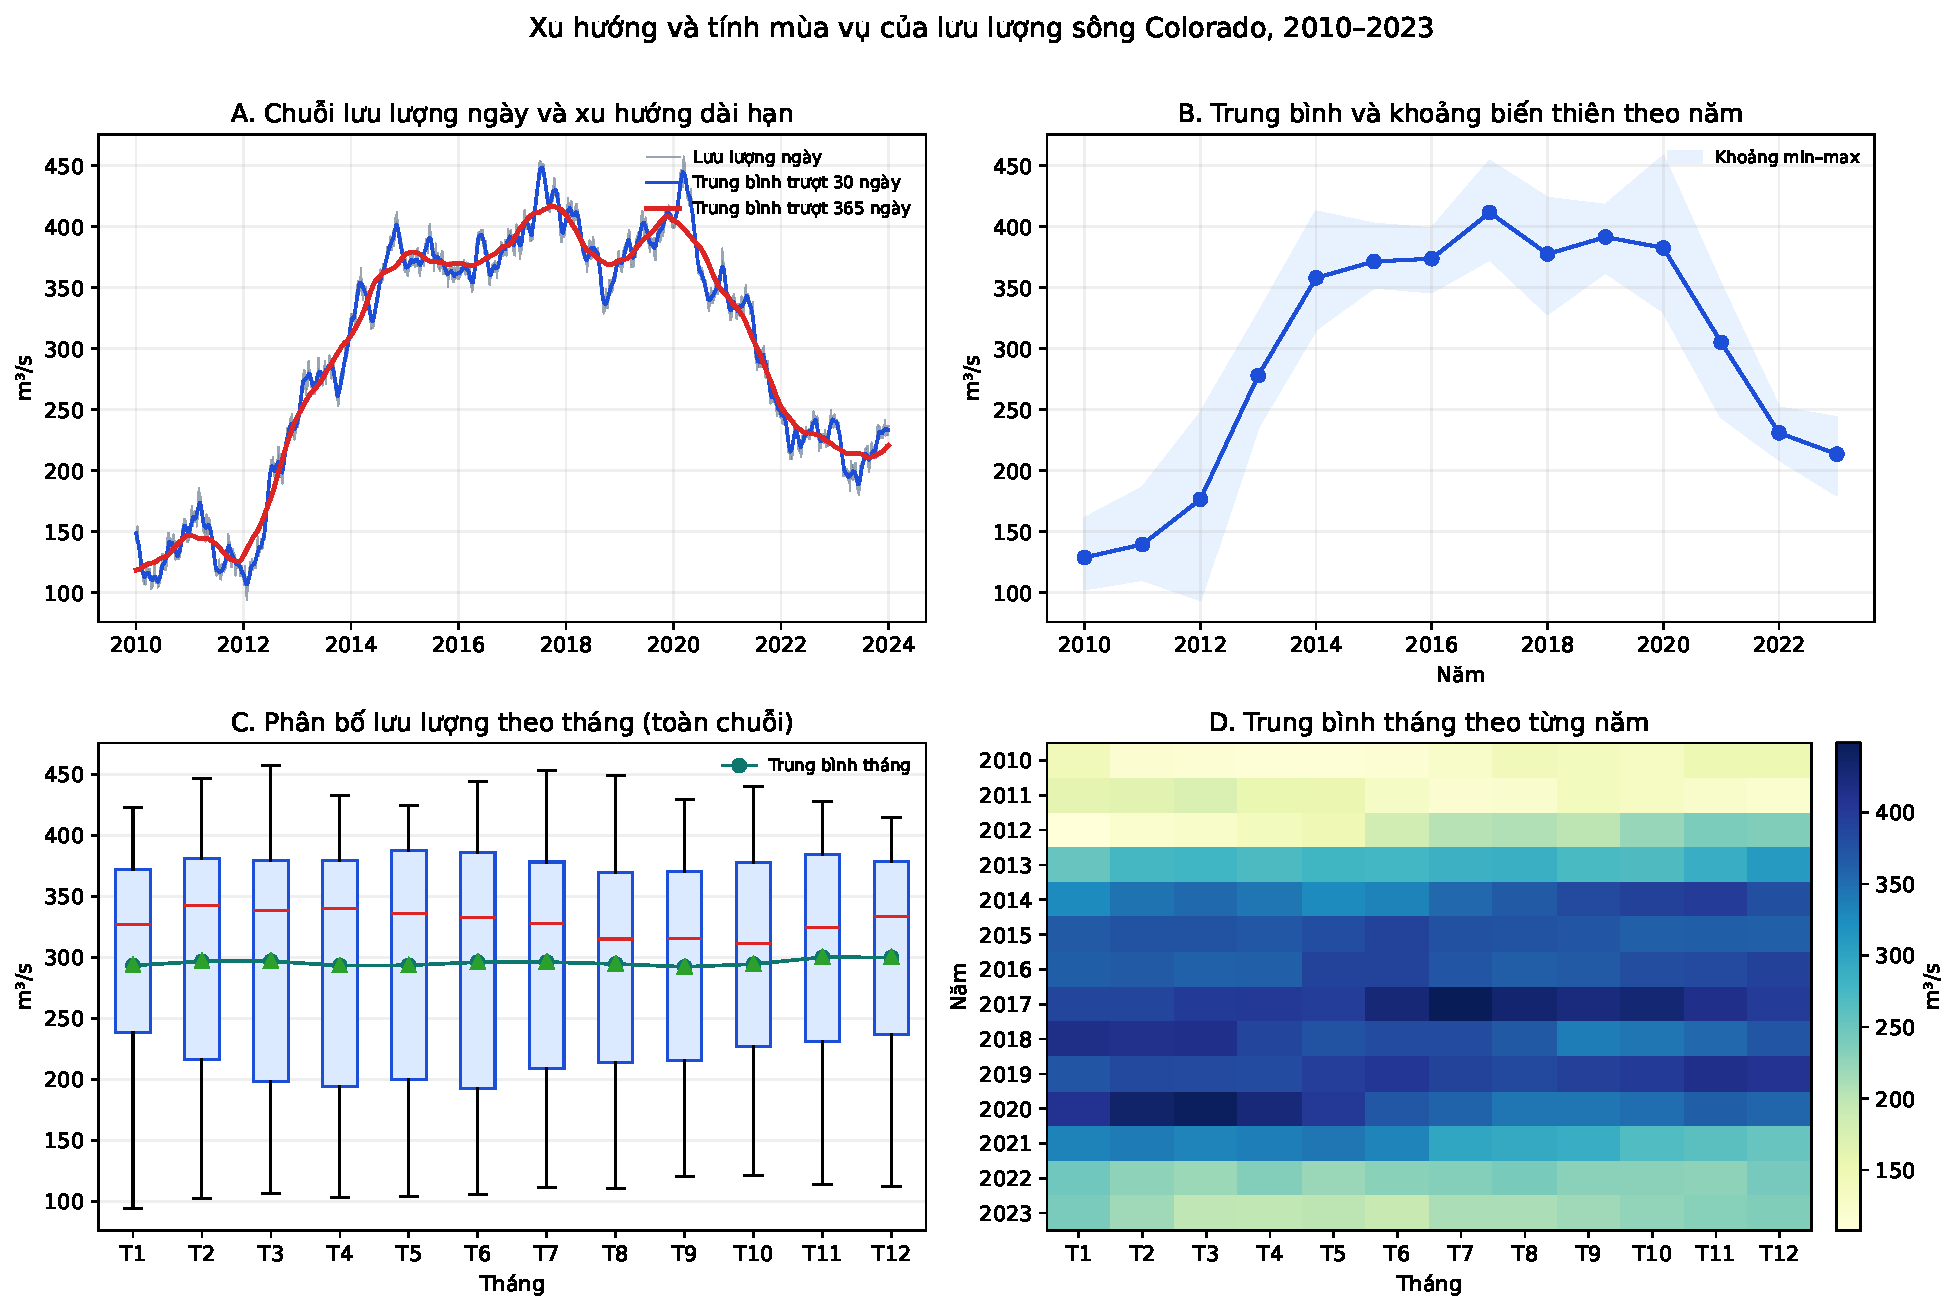
\includegraphics[width=0.86\linewidth]{figures/trend_seasonality.pdf}
\caption{Chuỗi lưu lượng ngày và thành phần xu hướng/mùa vụ. Mùa vụ gần như phẳng;
xu hướng thay đổi mạnh theo từng giai đoạn.}
\label{fig:q1}
\end{figure}

STL với chu kỳ 365 ngày và cấu hình robust cho seasonal strength \SeasonalStrength{}
và trend strength \TrendStrength. ACF lag 365 ngày là \AcfYear, rất gần 0; ACF lag 7
ngày và 30 ngày còn cao do tính liên tục ngắn hạn, không phải do mùa vụ năm. Vì vậy
không nên đọc chuỗi này như một mùa vụ đều đặn kiểu thủy văn ôn đới. Cần mô tả xu hướng
theo từng giai đoạn và nhấn mạnh các năm 2017--2019 có mức lưu lượng cao nổi bật.
